%%%%%%%%%%%%%%%%%%%%% chapter.tex %%%%%%%%%%%%%%%%%%%%%%%%%%%%%%%%%
%
% sample chapter
%
% Use this file as a template for your own input.
%
%%%%%%%%%%%%%%%%%%%%%%%% Springer-Verlag %%%%%%%%%%%%%%%%%%%%%%%%%%
%\motto{Use the template \emph{chapter.tex} to style the various elements of your chapter content.}


\chapter{Network-aware Adaptive LBT (NALT) Coexistence Mechanism}
\label{intro-NALT} % Always give a unique label
% use \chaptermark{}
% to alter or adjust the chapter heading in the running head

\abstract*{In the absence of coordination between radio access technologies (RATs), and with the goal of deploying unlicensed LTE without requiring changes to the \mbox{Wi-Fi} MAC layer, it falls to the LTE base stations to ensure fair coexistence. The multiple access method used in \mbox{Wi-Fi} is designed for fair sharing of the channel with devices operating towards the same goal. Following this paradigm, if \mbox{LAA-LTE} is not carefully designed to ensure fairness, it can easily lead to \mbox{Wi-Fi} stations being barred from the channel. The greatest gains in fair coexistence are achieved when \mbox{LAA-LTE} behaves in as \mbox{Wi-Fi}-like a manner as possible; however, this may not allow LTE to make the best use of the channel.  In this chapter, a network-aware adaptive LBT mechanism (NALT) is presented which passively monitors both channel conditions and usage activity to maximize transmission opportunities while respecting fair sharing of the channel, all in a way that is transparent to incumbent \mbox{Wi-Fi} devices. Simulation results are presented demonstrating the effectiveness of NALT in providing proportional fair sharing among \mbox{LAA-LTE} and \mbox{Wi-Fi} devices.}


In the absence of coordination between radio access technologies (RATs), and with the goal of deploying unlicensed LTE without requiring changes to the \mbox{Wi-Fi} MAC layer, it falls to the LTE base stations to ensure fair coexistence. The multiple access method used in \mbox{Wi-Fi} is designed for fair sharing of the channel with devices operating towards the same goal. Following this paradigm, if \mbox{LAA-LTE} is not carefully designed to ensure fairness, it can easily lead to \mbox{Wi-Fi} stations being barred from the channel. The greatest gains in fair coexistence are achieved when \mbox{LAA-LTE} behaves in as \mbox{Wi-Fi}-like a manner as possible; however, this may not allow LTE to make the best use of the channel.  In this chapter, a network-aware adaptive LBT mechanism (NALT) is presented which passively monitors both channel conditions and usage activity to maximize transmission opportunities while respecting fair sharing of the channel, all in a way that is transparent to incumbent \mbox{Wi-Fi} devices. Simulation results are presented demonstrating the effectiveness of NALT in providing proportional fair sharing among \mbox{LAA-LTE} and \mbox{Wi-Fi} devices.

\section{Background and Theoretical Basis}
\label{background}
As discussed in Chapter \ref{overview-wifi}, \mbox{\mbox{Wi-Fi}} employs a fairly simple multiple access strategy which can be easily overwhelmed if competing devices are not also designed for fair coexistence. The \mbox{\mbox{Wi-Fi}} MAC protocol employs listen-before-talk (LBT) and is based on a probabilistic model of channel access which minimizes collisions through the use of random backoff to limit the probability that two stations will transmit at the same time after the channel has become idle \cite{80211}.  When a collision is inferred after a failed transmission, the set of possible backoff values grows exponentially to further reduce the probability of subsequent transmission failures.  While the ETSI LBT standard, on which the recommended mechanism for \mbox{\mbox{LAA-LTE}} is based, is also probabilistic, it employs a random backoff from a fixed set of possible backoff values \cite{3gpp}, which does not attempt to reduce the probability of collision on repeated failed transmission.  Thus, if a collision occurs, \mbox{\mbox{Wi-Fi}} will react by reducing its probability of gaining access to the channel, while a device modelled on the ETIS LBT mechanism will maintain the same probability of channel access.  Additionally, \mbox{\mbox{LAA-LTE}} used for supplemental downlink or carrier aggregation is expected to align subframes with the licensed band, and such subframes have a duration of $1$ms, which can be significantly longer than the average channel occupancy time of a \mbox{Wi-Fi} station.  Combined, these two factors will lead to \mbox{\mbox{LAA-LTE}} stations both winning the channel more frequently, and then occupying the channel for significantly longer than an average competing \mbox{\mbox{Wi-Fi}} station would, even if the number of channel accesses were equal.  Since \mbox{\mbox{Wi-Fi}} stations may operate at any of several modulation and coding schemes, it is also difficult to provide throughput fairness across a large number of \mbox{Wi-Fi} devices. However, airtime fairness can be achieved by leveraging the principles developed for the $802.11$e Enhanced Distributed Channel Access (EDCA) function for service differentiation between traffic priorities in \mbox{Wi-Fi}.  

In EDCA, \mbox{\mbox{Wi-Fi}} parameters such as contention window and inter-frame spacing are set up to provide quality of service differentiation and priority enforcement between varying types of traffic \cite{80211}.  By changing these parameters, it is possible to impact the probability of channel access in a predictable way.  By constantly managing these parameters in response to network activity, it is possible to maintain long run proportionally fair sharing between the traffic categories or classes of devices on competing networks.  

Specifically, the relationship between minimum contention window size for two traffic classes, and their relative proportion of channel access has been found to be
\begin{equation}\label{cw}
\frac{\theta_i}{\theta_j} \approx \frac{CW^j_{min}}{CW^i_{min}}
\end{equation}
where, $\frac{\theta_i}{\theta_j}$ is the ratio of channel access $i$ sees relative to class $j$, and $CW^x_{min}$ is the minimum contention window used by class $x$ \cite{chou}\cite{yoon}.  

To use Eq. \ref{cw} to balance airtime between \mbox{\mbox{LAA-LTE}} and \mbox{\mbox{Wi-Fi}}, it is necessary to treat all \mbox{\mbox{Wi-Fi}} stations and all \mbox{LAA-LTE} networks as traffic classes and account for the duration of channel access for each class. Between the two traffic classes, this duration will generally be longer for \mbox{LAA-LTE} than for \mbox{Wi-Fi}, due to the synchronization between licensed and unlicensed transmissions and the range of data rates available for \mbox{Wi-Fi} stations over clean channels.  As such, \mbox{LAA-LTE} will receive fewer channel accesses in order to achieve the same airtime allocation. For example, if a \mbox{\mbox{Wi-Fi}} channel access takes half the time of a \mbox{\mbox{LAA-LTE}} channel access, in the case of a single \mbox{\mbox{LAA-LTE}} station competing with a single \mbox{\mbox{Wi-Fi}} station, the \mbox{\mbox{Wi-Fi}} station should receive twice as many transmission opportunities as the \mbox{\mbox{LAA-LTE}} station in order to achieve equal airtime.  If there were two \mbox{\mbox{Wi-Fi}} stations, in order for each to have equal airtime, the \mbox{\mbox{LAA-LTE}} station should receive one quarter as many transmission opportunities as the combined \mbox{\mbox{Wi-Fi}} stations, so that proportionally each of the three stations would receive equal airtime on average.  Adding a proportionality constant $\rho$, which is the ratio of \mbox{\mbox{LAA-LTE}} transmission time to average \mbox{\mbox{Wi-Fi}} transmission time, and solving Eq. \ref{cw} for the required $CW_{min}$ values to realize equal airtime yields,
\begin{equation}\label{cwlte}
CW^{LTE}_{min} = \rho\cdot{CW^{WiFi}_{min}}
\end{equation}
Since we seek equal airtime, we require that $\rho\cdot\frac{\theta_{WiFi}}{\theta_{LTE}} = 1$, or in other words, the \mbox{Wi-Fi} traffic class receives $\rho$ times as many channel accesses as the \mbox{LAA-LTE} class.

The relation in Eq. \ref{cwlte} provides an approximation of the optimal $CW^{LTE}_{min}$ to provide airtime fairness; however, the \mbox{\mbox{Wi-Fi}} traffic class may be made up of stations which are using different transmission rates and $CW_{min}$ values. In order to estimate the $CW^{WiFi}_{min}$ to use in Eq. \ref{cwlte}, and adjust to changing network topologies, an estimate of the average current \mbox{Wi-Fi} contention window being used is required.  Such an estimate can be obtained from the relationship between contention window and the probability of collision. For \mbox{\mbox{Wi-Fi}} networks, the probability of collision, $p$, in a saturated network is given by, 

\begin{equation}\label{pcollision}
p = 1-(1-\sfrac{1}{CW_{avg}})^{n-1}
\end{equation}
where $CW_{avg}$ is the average contention window currently being employed in the network, and $n$ is the number of competing stations \cite{vu}.  Rearranging and solving for $CW_{avg}$ yields,
\begin{equation}\label{cwavg}
CW_{avg} = \frac{1}{1-e^{ \sfrac{ln(1-p)}{(n-1)} }}
\end{equation}
Eq. \ref{cwavg} provides the average contention window size for all stations, both \mbox{LAA-LTE} and \mbox{Wi-Fi}, i.e. $n = n_{WiFi} + n_{LTE}$.  In order to consider only the average contention window size for the \mbox{\mbox{Wi-Fi}} stations, and noting the optimal $CW^{LTE}_{min}$ to $CW^{WiFi}_{min}$ ratio, we can estimate $CW^{WiFi}_{min}$ as
\begin{equation}\label{cwwifi}
CW^{WiFi}_{avg} = CW_{avg}\left ( \frac{n_{WiFi} + n_{LTE}}{n_{WiFi} + \rho\cdot n_{LTE}} \right )
\end{equation}
Combining Eq. \ref{cwlte} through Eq. \ref{cwwifi},  we set 
\begin{equation}\label{cwlteopt}
CW^{LTE} = \rho \cdot{CW^{WiFi}_{avg}} = \frac{\rho}{1-e^{ \sfrac{ln(1-p)}{(n_{WiFi} + n_{LTE}-1)} }}\left ( \frac{n_{WiFi} + n_{LTE}}{n_{WiFi} + \rho\cdot n_{LTE}} \right )
\end{equation}

Adapting the contention window used in each \mbox{LAA-LTE} network according to Eq. \ref{cwlteopt} will provide proportional fair channel access across the two classes of devices in the long run.  In order to make use of this relation, the \mbox{LAA-LTE} base stations must know, or be reasonably able to estimate, the probability of collision in the network, $p$, as well as the number and type of competing devices.  

\section{Proposed Mechanism}
\label{proposed}
NALT is defined as a simple, distributed coordination function to be implemented by \mbox{LAA-LTE} base stations.  This allows several \mbox{LAA-LTE} networks to effectively and independently fairly share the channel with both each other and incumbent \mbox{Wi-Fi} stations, without any changes being required in the \mbox{Wi-Fi} stations.

To make use of the relationships in the previous sections, the following assumptions are made:
\begin{itemize}
	\item NALT-enabled base stations are able to:
	\begin{itemize}
	\item Analyze traffic on the channel and determine the number of competing stations and their types
	\item Determine average transmission durations either by decoding transmission headers, actively timing the transmissions, or some other suitable mechanism
	\end{itemize} 
	\item Successfully gaining access to the channel means that the transmission was successful, i.e. ignoring noise sources and the hidden terminal problem, which NALT does not attempt to address
	\item Failed \mbox{\mbox{LAA-LTE}} transmissions on unlicensed channels can be reported to the base station on control channels in the licensed spectrum
	\item Collisions experienced on the \mbox{LAA-LTE} network occur with approximately the same probability as collisions experienced by \mbox{Wi-Fi} stations
\end{itemize}

In order to use Eq. \ref{cwlteopt} in an implementable algorithm, the probability of collision  $p$ and the number of competing \mbox{Wi-Fi} stations and \mbox{LAA-LTE} networks are required. Since these values cannot be known beforehand, the number of competitors is learned over time and the required probability of collision is estimated in each NALT-enabled \mbox{LAA-LTE} network as the ratio of observed \mbox{\mbox{LAA-LTE}} collisions to the number of \mbox{\mbox{LAA-LTE}} channel uses, on a network by network basis.  Noting that this is an empirical estimate of the true statistic, its reliability is inversely proportional to the number of samples and, although it improves over time, it must be considered highly suspect for a limited number of samples and be restricted to some reasonable range. 

The relationship in Eq. \ref{cwlteopt} is exploited to achieve fair airtime allocation by tuning the $CW_{min}$ values used by competing stations in each \mbox{LAA-LTE} network.  Since it is desired to avoid any changes to \mbox{\mbox{Wi-Fi}}, and fairer coexistence can be achieved by designing a more \mbox{``\mbox{\mbox{Wi-Fi}}-like"} MAC layer for \mbox{\mbox{LAA-LTE}}, the contention window used by \mbox{\mbox{LAA-LTE}} must increase as the number of collisions increases.  To facilitate fair airtime allocations across all competing devices, the contention window should follow Eq. \ref{cwlteopt}.  Based on the limitations of the estimates employed, and to ensure that the contention window stays within reasonable bounds, the maximum and minimum values for $CW^{LTE}$ are chosen to match the range of possible values for \mbox{\mbox{Wi-Fi}} \cite{80211}.  

Combining these requirements and the preceding equations and assumptions, at each time instance an \mbox{\mbox{LAA-LTE}} station will estimate the average \mbox{\mbox{Wi-Fi}} contention window as follows:
\begin{align}
CW^{WiFi}_{avg} = CW^{WiFi}_{min}, \text{  if \{ \# of \mbox{\mbox{Wi-Fi}} Tx\}$> \rho\cdot$\{  \# of \mbox{\mbox{LAA-LTE}} Tx\}}\notag\\ 
\text{Otherwise, update according to Eq. \ref{cwwifi}.}
\end{align}
\mbox{\mbox{LAA-LTE}} will follow the same backoff procedure as \mbox{\mbox{Wi-Fi}} by increasing its contention window after a collision according to
\begin{align}
&CW^{LTE}=\;\;min\left[max\left(CW^{LTE}*2,\rho \cdot CW^{WiFi}_{avg}\right), CW^{LTE}_{MAX}\right]
\end{align}
and decreasing its contention window after a successful transmission according to 
\begin{align}
&CW^{LTE}=\;\;min\left[max\left(CW^{LTE}_{MIN},\rho \cdot CW^{WiFi}_{avg}\right), CW^{LTE}_{MAX}\right]
\end{align}

These equations, in addition to function for gathering channel usage statistics are implemented in each of the competing \mbox{LAA-LTE} eNBs.  This mechanism requires no explicit coordination between the \mbox{LAA-LTE} base stations nor any changes to \mbox{Wi-Fi} stations. The operation of NALT is depicted in Fig. \ref{NALT-flowchart}. 
\begin{figure}[!ht]
	\centering
	\includegraphics[width=\textwidth]{figs/NALT-flowchart}
	\caption{Network-aware Adaptive LBT algorithm.}
	\label{NALT-flowchart}
\end{figure}%Works in grayscale
The operation is divided into three main functions: Learning, where the NALT-enabled eNB learns about the other occupants of the network and their transmission profiles; Transmission, which follows a random back off interval; and Adaptation, which uses the gathered data and employs exponential backoff to ensure fair coexistence.


\section{Performance Evaluation}\label{perf-eval}
To evaluate the performance of NALT, a high-level MATLAB simulation was developed in which the proportion of successful channel accesses achieved by each class of devices was tracked. Since NALT is an adaptive medium access strategy, the simulation looks only at the proportion of successful channel accesses, and assumes all attempted transmissions only fail if a collision occurs.  That is, other interferences sources and problems such as hidden terminals, are ignored.  The ETSI LBT mechanism was simulated as a benchmark against which the effectiveness of NALT was compared.


\subsection{System Model}
\label{sys-model}
The system includes a number of NALT-enabled \mbox{LAA-LTE} networks interacting with a varying number of \mbox{Wi-Fi} devices.  \mbox{LAA-LTE} transmissions in the unlicensed bands are expected to be aligned with the LTE-A frames in the licensed spectrum, thus it can be assumed that \mbox{\mbox{LAA-LTE}} user equipment (UE) will be coordinated via licensed control channels, with scheduling done by the eNB so that there is coordinated channel accesses for both uplink and downlink traffic.  The system model incorporates this by assuming the eNB will not schedule either its own DL transmission or two UE UL transmissions in the same time-frequency slot, so that the only sources of collisions are from \mbox{Wi-Fi} stations and other \mbox{LAA-LTE} networks. Thus, each simulated \mbox{LAA-LTE} device in fact represents an independent network of \mbox{LAA-LTE} devices which are not required to contend with each other. Additionally, although the NALT-enabled eNB would be capable of analyzing traffic on the channel to determine the average \mbox{Wi-Fi} transmission parameters, such as bitrate and channel occupancy time, for simplicity, we assume that both UE and \mbox{\mbox{Wi-Fi}} stations use the same modulation and coding scheme and channel bandwidth, resulting in a data rate of $135$ Mbps.  Other than the adaptive contention window, the \mbox{LAA-LTE} channel occupancy and minimum idle time were modelled after ETSI LBE LBT and the proposed mechanisms for \mbox{\mbox{LAA-LTE}} \cite{3gpp}.  The other pertinent simulation parameters are listed in Table \ref{params}.
\begin{table}
	\caption{NALT Simulation Parameters}
	\label{params}      
	\begin{tabular}{p{0.7\textwidth}p{0.28\textwidth}}
		\hline\noalign{\smallskip}
		Parameter & Value \\
		\noalign{\smallskip}\svhline\noalign{\smallskip}
		Number of competing \mbox{\mbox{Wi-Fi}} stations& $1 - 15$ \\ 
		\mbox{Wi-Fi} OFDM Symbol Duration (slot) & 9 $\mu$s    \\ 
		DCF Interframe Spacing $^1$ & 34 $\mu$s   \\ 
		Short Interframe Spacing$^1$ & 16 $\mu$s   \\ 
		\mbox{\mbox{Wi-Fi}} Frame Size & 1536 bytes  \\ 
		\mbox{\mbox{Wi-Fi}} Tx Duration$^2$ (Frame Tx + SIFS +ACK) & 198 $\mu$s   \\ 
		Number of independent LTE Networks & 1, 5 \\
		\mbox{\mbox{LAA-LTE}} Channel Occupancy Time  & 1000 $\mu$s \\ 	
		\noalign{\smallskip}\hline\noalign{\smallskip}
	\end{tabular}
	$^1$ Defined inter-frame spacing per 802.11n operating in the 5 GHz band \\
	$^2$ Based on header transmitted at lowest supported rate and remaining frame at specified bitrate	 
\end{table}

\subsection{Simulation Results}
\label{sim-results}
NALT is a probabilistic coexistence mechanism, so to evaluate the fairness provided by NALT the average of numerous trials were considered.  Network topologies of between $1$ and $15$ \mbox{\mbox{Wi-Fi}} stations contending with \mbox{\mbox{LAA-LTE}} networks were examined and the proportion of successful channel accesses for each class of devices, related to airtime by the class' transmission duration, was tracked across all trials.  

Initially, NALT was tested with a single \mbox{LAA-LTE} network competing with between 1 and 15 \mbox{Wi-Fi} stations.  The resulting proportion of airtime for each device when using NALT is shown in Fig. \ref{basic-results}.
\begin{figure}[!ht]	
	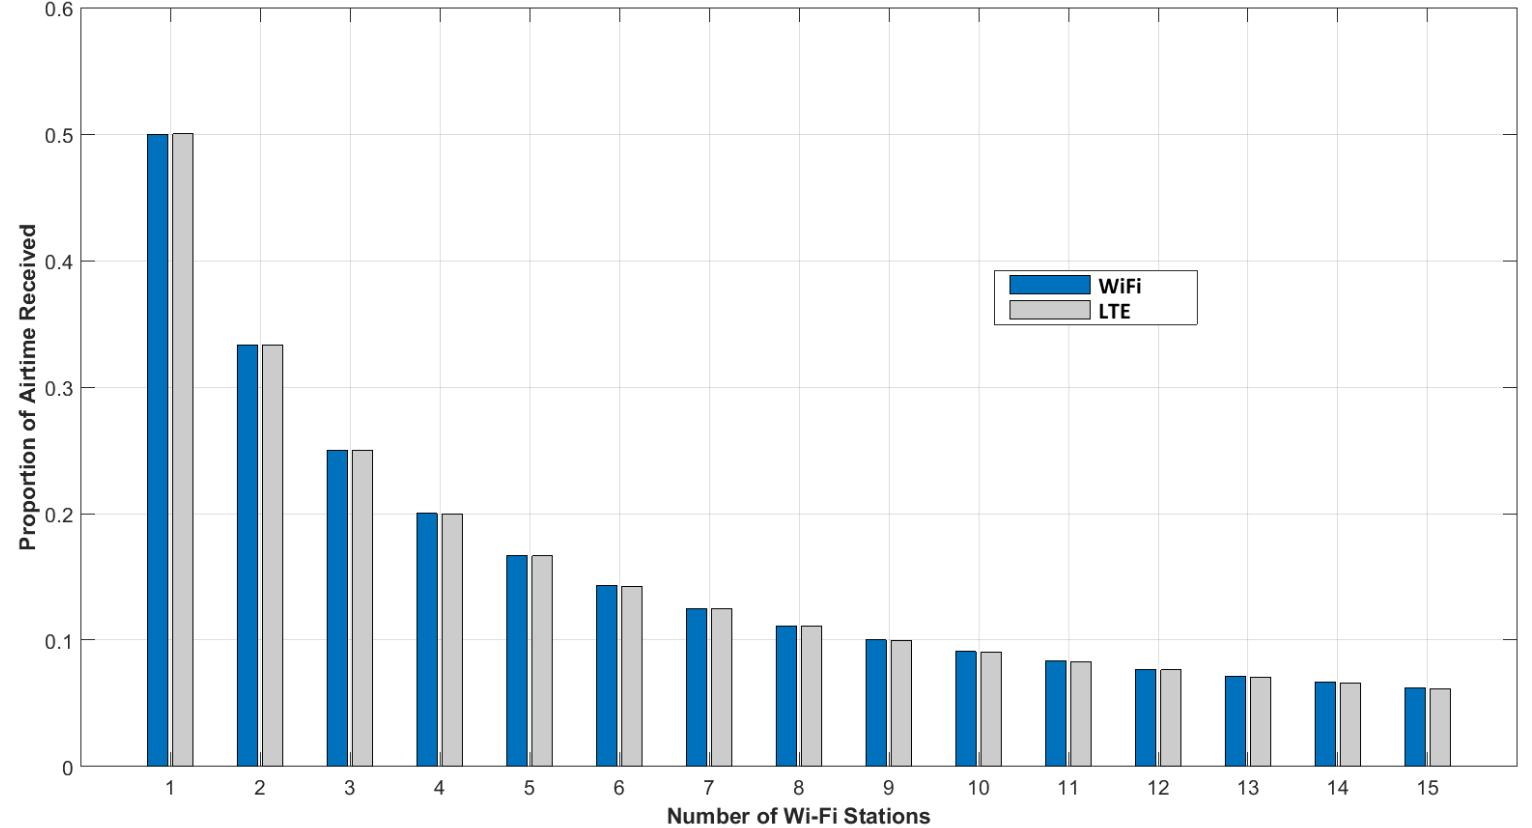
\includegraphics[width=\textwidth]{figs/NALT-1-15}
	\caption{Airtime allocations for each station with \mbox{LAA-LTE} using NALT.}
	\label{basic-results}
\end{figure}
In each configuration, fair sharing was achieved, with every member of each class receiving a proportional airtime allocation. 

For comparison, the simulation was run with the same parameters as in Table \ref{params}, but with a fixed contention window size of $16$, corresponding to the midpoint of possible values under ETSI LBE LBT \cite{3gpp}. The resulting airtime allocations, normalized to the number of devices, are shown in Fig. \ref{compresults}.
\begin{figure}[!ht]
	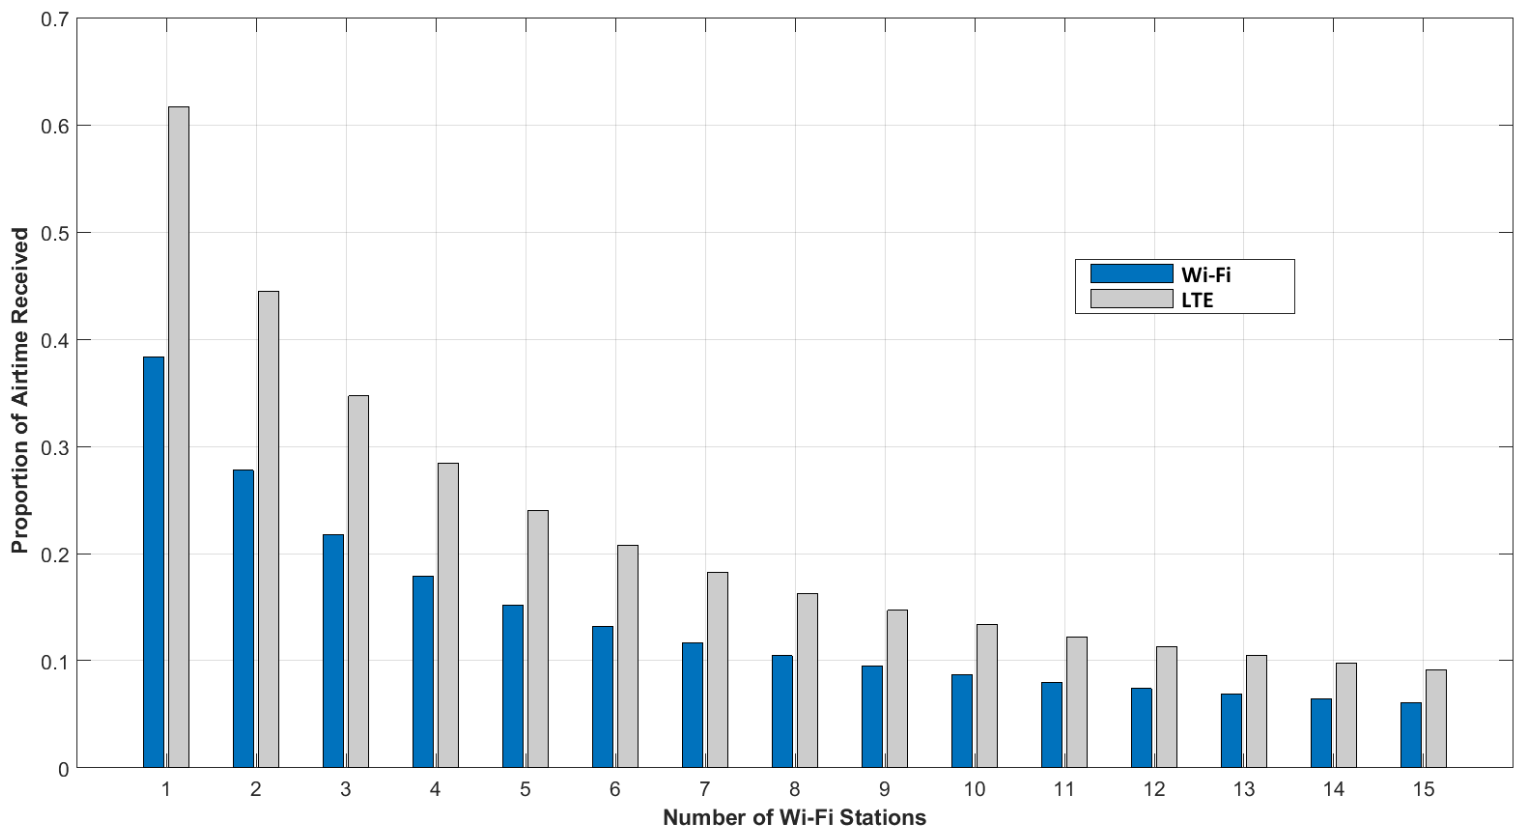
\includegraphics[width=\textwidth]{figs/ETSIforComp}
	\caption{Airtime allocations for each station with \mbox{LAA-LTE} using ETSI LBE LBT.}
	\label{compresults}
\end{figure}
As expected, \mbox{LAA-LTE} transmission receive a disproportionately high airtime allocation compared to Wi-FI.  This is a result of the static contention window used in ETSI LBT providing an increasingly higher proportion of channel accesses as collisions on the channel occur and the \mbox{Wi-Fi} contention window grows.

Since it is likely that \mbox{LAA-LTE} networks will be deployed alongside other competing \mbox{LAA-LTE} networks, the simulation was extended to evaluate the effectiveness of NALT under these conditions.  The simulation was run with 5 independent NALT-enabled \mbox{LAA-LTE} networks competing against each other as well as \mbox{Wi-Fi} stations.  The resulting proportion of airtime for each device when using NALT is shown in Fig. \ref{multi-results}.
\begin{figure}[H]	
	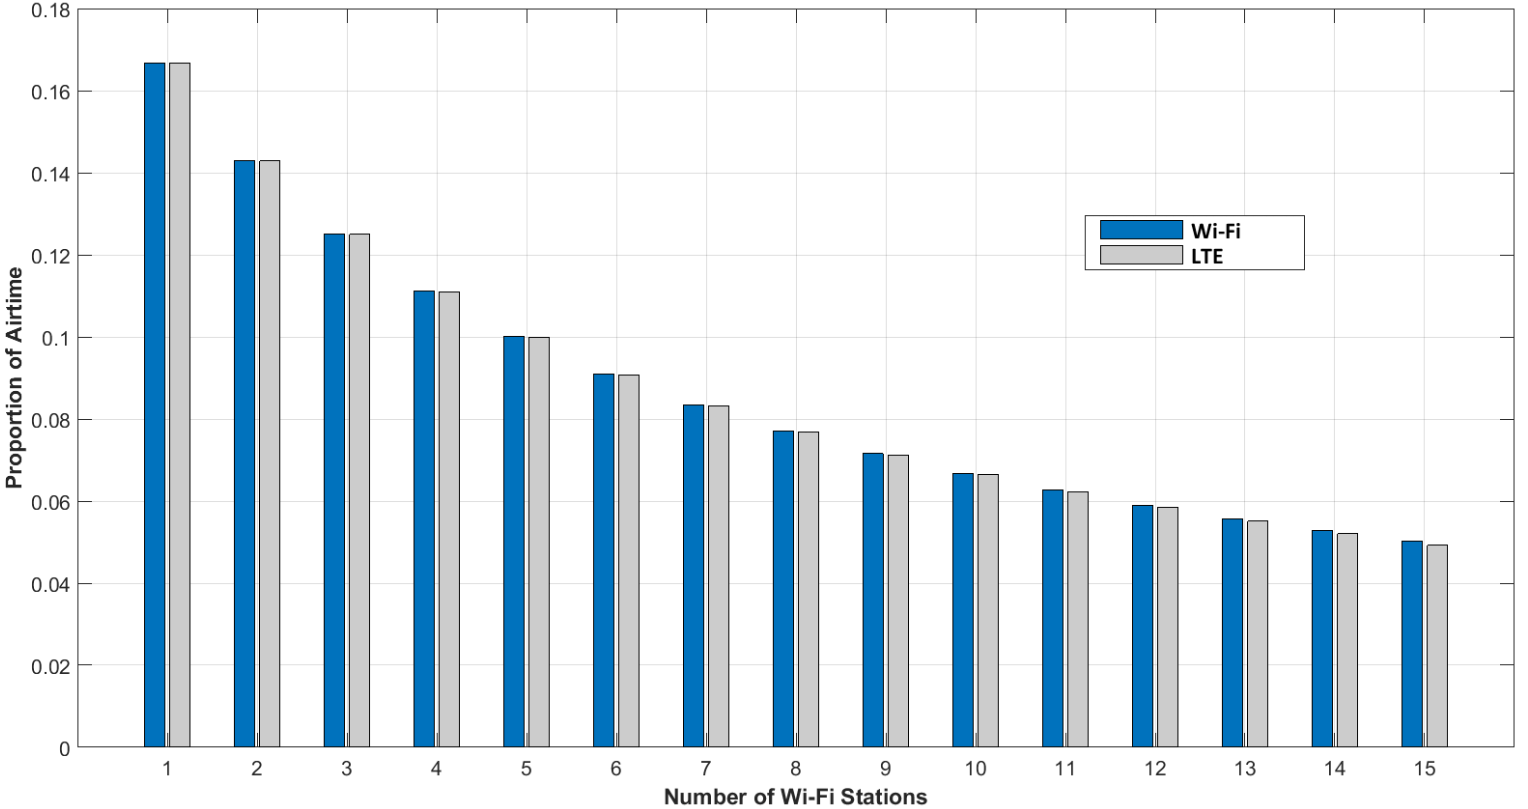
\includegraphics[width=\textwidth]{figs/NALT-5-15}
	\caption{Airtime allocations for each station with five \mbox{LAA-LTE} networks using NALT.}
	\label{multi-results}
\end{figure}

It is further conceivable that \mbox{LAA-LTE} networks will be deployed where there are either no competing \mbox{Wi-Fi} stations, or the level of interference between the RATs is negligible.  Fig. \ref{NALT-only-results}, shows the resulting fair allocation of airtime for each device when NALT is used in a \mbox{LAA-LTE} only deployment. 
\begin{figure}[H]
	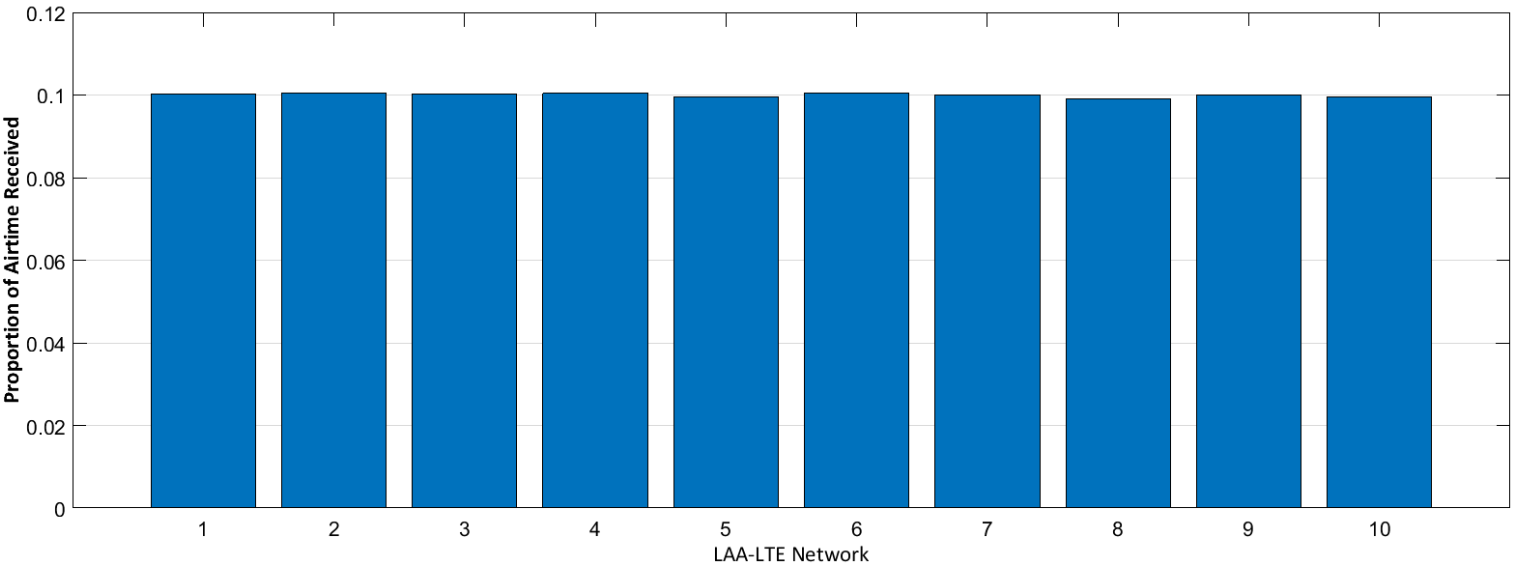
\includegraphics[width=\textwidth]{figs/LAAonly}
	\caption{Airtime allocations from \mbox{LAA-LTE} only channel contention when using NALT.}
	\label{NALT-only-results}
\end{figure}

\section{Discussion and Future Work}
\label{future-work}
NALT requires no changes to \mbox{\mbox{Wi-Fi}} devices, and high-level simulation results show promise in providing fair coexistence in several deployment scenarios.  In each of the cases examined, NALT provides approximately equal airtime to each station, regardless of type or how many competing stations exist.  

As noted, several simplifying assumptions were made, which may affect the results.  It is reasonable that \mbox{\mbox{LAA-LTE}} would be able to analyze the channel and determine the number or competing \mbox{\mbox{Wi-Fi}} stations as well as their transmission profiles, from the \mbox{\mbox{Wi-Fi}} preamble and MAC header; however a learning period to gather sufficient data to make reasonable estimates of the averages may or may not be necessary.  If necessary, it may negatively impact overall performance. It is desirable to implement the learning functions depicted in Fig. \ref{NALT-flowchart} and determine if the processing overhead could reasonably meet the timing constraints. Further, the assumption was made that all \mbox{\mbox{Wi-Fi}} stations use the same data rate, and hence have the same transmission duration for standard size frames.  The potential impacts of using an average \mbox{\mbox{Wi-Fi}} transmission duration in a multi-rate \mbox{\mbox{Wi-Fi}} network has not explored.   Finally, the impacts of hidden terminals, non-saturated stations, and lossy channels, were not considered, and may have interesting implications. 

%%%%%%%%%%%%%%%%%%%%%%%% referenc.tex %%%%%%%%%%%%%%%%%%%%%%%%%%%%%%
% sample references
% %
% Use this file as a template for your own input.
%
%%%%%%%%%%%%%%%%%%%%%%%% Springer-Verlag %%%%%%%%%%%%%%%%%%%%%%%%%%

\begin{thebibliography}{99.}%
	\bibitem{3gpp}{3GPP}, ``Feasibility study on licensed-assisted access to unlicensed spectrum,'' \emph{{TR 36.889 v13.0.0}}, July 2015.
	\bibitem{chou} C.~T. Chou, K.~G. Shin, and S.~Shankar, ``{Contention-based airtime usage control in multirate IEEE 802.11 wireless LANs},'' \emph{{IEEE/ACM Transactions on Networking}}, vol.~14, no.~6, pp. 1179--1192, December 2006.	
	\bibitem{80211}``{IEEE Standard for information technology--Telecommunications and information exchange between systems Local and metropolitan area networks--Specific requirements Part 11: Wireless LAN medium access control (MAC) and physical layer (PHY) specifications},'' \emph{{IEEE Std 802.11-2012 (Revision of IEEE Std 802.11-2007)}}, pp. 818--972, March 2012.	
	\bibitem{vu} H.~L. Vu and T.~Sakurai, ``{Collision probability in saturated IEEE 802.11 networks},'' in \emph{{Australian Telecommunication Networks \& Applications Conference}}, September 2006, pp. 1--5.
	\bibitem{yoon} {J. Yoon, S. Yun, et al}, ``{Maximizing differentiated throughput in IEEE 802.11e wireless LANs},'' in \emph{{ Proceedings of the 31st IEEE Conference on Local Computer Networks}}, vol.~14, no.~6, November 2006, pp. 411--417.
\end{thebibliography}


